\documentclass{beamer}

\title{Isabelle/HOL on Fork Prevention\\ in the Coming Ethereum Protocol}
\author{Yoichi Hirai\\ {\small Ethereum Foundation}}
\date{Berlin, 30 Aug. 2017}

\begin{document}

\begin{frame}
\titlepage
\end{frame}

\begin{frame}{What is Ethereum}

Ethereum is one-instance of a virtual machine
\begin{itemize}
\item as powerful as a 20-year-old smart phone
\item replicated globally
\item with no central parties
\item running for 2 years by now
\end{itemize}

\vfill

How does Ethereum synchronize execution traces? \\
Asynchronous communication cannot establish new common knowledge.
\end{frame}

\begin{frame}{Blockchain}
is just a data strucuture.  It is a tree, not a chain.

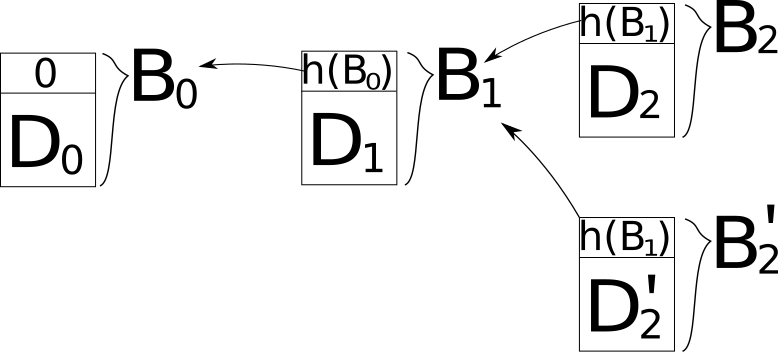
\includegraphics[width=\textwidth]{blockchains.png}

A small number $h(B_n)$ identifies a sequence $B_0, \ldots B_n$ and \\
moreover, in Ethereum, the execution trace of a virtual machine.

\end{frame}


\begin{frame}{Proof of Work}

\begin{itemize}
\item a block's content $D$ needs to contain a nicely chosen nonce\\ so that the hash $h(D)$ of the block is small enough
\item when you find such a nonce, the protocol gives reward in your account (in the state after the block)
\item account?
\end{itemize}

Finding a good nonce is called \structure{mining}.

I belive nobody has found a better way than brute-force.
\end{frame}

\begin{frame}{Proof of Work}

\structure{If you succeed creating a block}
\begin{enumerate}
\item the block reward is only spendable in chains that include your block
\item you should send around the block, maybe
\end{enumerate}

\structure{If you see a block being sent around}
\begin{enumerate}
\item if that's the best block you've seen, you should try to mine on the block \\
      (assumption: absense of complicated motives, other nodes' straightforward behavior)
\item you should broadcast the block you are mining on, maybe
\end{enumerate}

\structure{Does it work?}  Yes, see Bitcoin.

\structure{Why?}  I don't know, honestly.
\end{frame}

\begin{frame}{Evaluating Proof of Work}

No good properties distributed-computation-wise.

(A good leader-election protocol can tolerate less than 1/3 Byzantine nodes.)

\structure{One Byzantine node can}
\begin{itemize}
\item be lucky enough to guess the secret keys of all public keys it sees.
\end{itemize}

\structure{One (economically) irrational node can}
\begin{itemize}
\item buy lots of machines to mine quicker than anybody, rewriting the history from any point.
\end{itemize}

\structure{Why would anybody choose this?} \underline{number of nodes} is not reliable.

Instead, Proof-of-Work uses electricity consumption (or luck).

Instead, Proof-of-Stake uses in-protocol deposit.

These designs require numbers that carry values.

\end{frame}


\begin{frame}{Proof-of-Stake}

\begin{itemize}
\item Replacing GPU and electricity with deposits of in-protocol tokens.
\item A difference: in-protocol tokens duplicate as forks happen.
\item Solution: provably dishonest behavior is punished on all forks.
\end{itemize}

\alert{Slash those who produce blocks on multiple chains!}\\ is too intimidating.
\end{frame}


\begin{frame}{I Received a Challenge: Original Text}

  \structure{Message types}

  \begin{itemize}
  \item commit(HASH, view)
  \item prepare(HASH, view, view\_source),\\ -1 $\le$ view\_source < view
  \end{itemize}

  \structure{Slashing conditions}

  \begin{enumerate}
    \item commit(H, v) REQUIRES 2/3 prepare(H, v, vs) for some consistent vs
    \item prepare(H, v, vs) REQUIRES 2/3 prepare(H\_anc, vs, vs') for some consistent vs', where H\_anc is a (v-vs)-degree ancestor of H, UNLESS vs = -1
    \item commit(H, v) + prepare(H, w, u) ILLEGAL if u < v < w
    \item prepare(X1, v, vs1) + prepare(X2, v, vs2) ILLEGAL unless X1 = X2 and vs1 = vs2
  \end{enumerate}

\end{frame}

\begin{frame}{Challenge Continued}

  \structure{Accountable safety argument}\\ (proof path - assume two incompatible values got committed, show 1/3+ SLASHED)

  \structure{Case 1}

\quad 2/3 commit(X, v) \& 2/3 commit(Y, v)

$\rightarrow$ 2/3 prepare(X, v, vs) \& 2/3 prepare(Y, v, vs')  (\structure{1.})

$\rightarrow$ 1/3 SLASHED (\structure{4.})

\structure{Case 2}

\quad 2/3 commit(Y, v2) \& 2/3 commit(X, v1),\\ Y is NOT a (v2-v1)-degree descendant of X, define Y[i] to be the ancestor of Y in view i

$\rightarrow$ 2/3 prepare(Y[v2], v2, vs), vs < v2 (\structure{1.})

$\rightarrow$ 2/3 prepare(Y[vs], vs, vs') (\structure{2.})

$\rightarrow$ ...

[continue induction until vs' < v1]

(Two base cases follow.)

\end{frame}

\begin{frame}{Alloy modelling}
Being unsure what the definitions meant, I turned to Alloy.

Alloy \url{url} is a tool based on relational-algebra.

You can type in definitions, assumptiions and a conjecture.

Alloy tries to find a counterexample.  No guarantees of false-negatives.
\end{frame}

\begin{frame}[fragile]{Alloy example}

\begin{verbatim}
module minimalt

sig View {
  v_prev: lone View // associated with at most one View called v_prev
}

sig Hash {
  h_prev: lone Hash
}

fact {
  no x : Hash | x in x.(^h_prev)
}

sig Prepare {
  hash : Hash,
  view: View,
  view_src : View
}

fact {
   all p : Prepare | p.view_src in (p.view.(^v_prev))
}

pred some_prepare {
   some Prepare
}

run some_prepare for 3
\end{verbatim}

\end{frame}

\begin{frame}
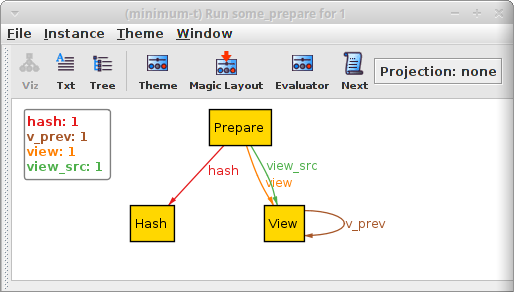
\includegraphics{circle.png}
\end{frame}

\begin{frame}{First attempt}
\end{frame}

\begin{frame}{Second attempt}
\end{frame}

\begin{frame}{Third attempt}
\end{frame}

\begin{frame}{Isabelle/HOL}
\alert{Turned out terse but followable in Isabelle/HOL (1,800 lines).}

\end{frame}

\begin{frame}{Fork}
\end{frame}

\begin{frame}{Exists something}
\end{frame}

\begin{frame}{Exists something something}
\end{frame}


\begin{frame}{Other formal verification projects}

\begin{itemize}
\item eth-isabelle: an executable specification of Ethereum Virtual Machine in Lem: available for Isabelle/HOL too.
\item some ongoing work on EVM1.5
\end{itemize}


\end{frame}

\end{document}
